% !TeX spellcheck = en_US

\chapter{Related Work}
\label{ch:related}

\section{Earlier Work Within The Providentia Project}
\label{sec:related-leon}

This work is deeply rooted in the earlier groundwork which was laid out for the \textit{Mono3D} task in highway scenarios~\cite{leonthesis} in the scope of the Providentia project.
Our earlier work took inspiration from the \textit{Cooperative Vehicle Infrastructure System}~\cite{guo2021detection} in the design and implementation of the two-stage detector based on the bottom contour of the vehicle instance mask, but also differs in key aspects.
The detection flow of our early \textit{Mono3D} highway detector is illustrated in figure~\ref{fig:related-leon}.

\begin{figure}[htb]
    \centering
    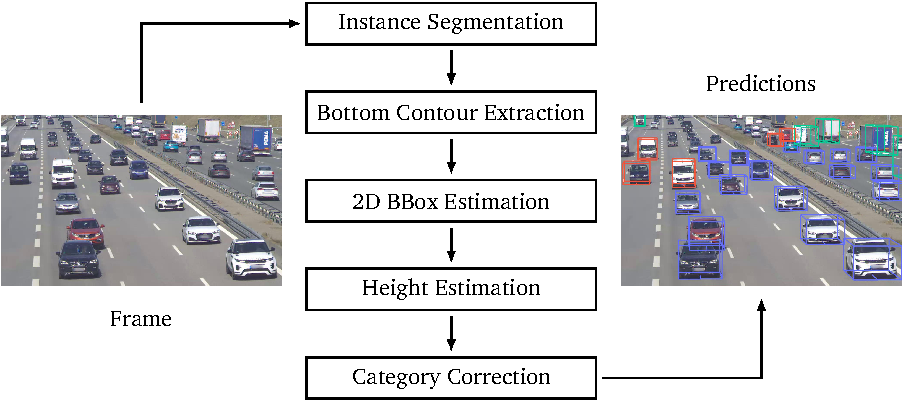
\includegraphics[width=0.9\linewidth]{figures/thesis_leon_fig_4_1}
    \caption{Figure 4.1 from~\cite{leonthesis}, illustrating the stages of the monocular 3D detection process for highway scenes.}
    \label{fig:related-leon}
\end{figure}

Note, that while this work adopts the first two elements of the detection flow \textemdash \textit{Instance Segmentation} and \textit{Bottom Contour Extraction} \textemdash we have completely reengineered all subsequent processes.
This earlier detector works well on highways, because it assumes a fixed orientation for all vehicles.
This also allows for a very straight-forward linear equation to solve for vehicle heights given their distance from the camera, as well as their instance mask heights.
In this work, the vehicle orientation is dynamically derived from the HD map and the vehicle's positional history.
The height estimation algorithm is revised accordingly.

\section{Detection of Vehicles in Cooperative Vehicle Infrastructure Systems}
\label{sec:related-coopvis}

The earlier Providentia highway detector was inspired by the \textit{Cooperative Vehicle Infrastructure System (CVIS)}~\cite{guo2021detection}, which also uses a two-stage detector with a $2D \rightarrow 3D$ lifting stage based on the vehicle bottom contour.
Their approach is illustrated in figure~\ref{fig:related-cvis}.

\begin{figure}[htb]
    \centering
    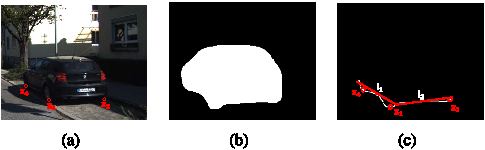
\includegraphics[width=1.0\linewidth]{figures/cvis_figure}
    %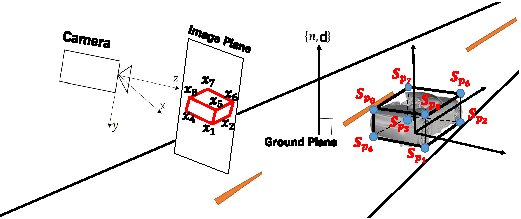
\includegraphics[width=0.39\linewidth]{figures/cvis_figure_2}
    \caption{Figure 1 from~\cite{guo2021detection}, illustrating their approach to keypoint estimation based on two lines which are regressed to the vehicle bottom contour: \textit{(a)} RGB image; \textit{(b)} vehicle segmentation mask; \textit{(c)} the contour point of the bottom edge of the vehicle and the contact points between vehicle and ground are represented by white dots and red circles.}
    \label{fig:related-cvis}
\end{figure}

While their approach has provided the basis for our research on \textit{Mono3d} in the Providentia project, it exhibits some flaws which we are hoping to have overcome (to some extent) in this work:

\begin{enumerate}
    \item Previous frames are not considered when a vehicle pose is estimated, potentially leading to bad yaw angle choices in ambiguous situations.
    \item They do not mention the effects shadows or noise due to obstructions or weather on their bottom contour line regression algorithm.\ The L-Shape-Fitting algorithm which is used in this work might be more robust in such situations, especially since we also apply \textit{DBSCAN}-based outlier filtering on the bottom contour.
    \item Their height estimation solution assumes that the closest vehicle top corner and bottom corner have the same depth from the camera, which leads to \textit{leaning} boxes in traffic monitoring situations where the camera is stationed highly above the vehicles.
    \item They do not consider non-vehicle \textit{Vulnerable Road Users (VRUs)} in their detector, such as bicyclists or pedestrians.\ This work is also detecting VRUs.
\end{enumerate}

Last but not least, no code is available for their approach.
This inherently necessitates research to reproduce their results.

\section{The L-Shape Fitting Method for Vehicle Pose Detection}
\label{sec:related-lshape-fitting}

Branching off \textit{CVIS}, this work (like~\cite{leonthesis}) makes use of \textit{L-Shape-Fitting (LSF)} to estimate vehicle size and orientation from the instance mask bottom contour.
This approach can also be interpreted as a \textit{pseudo-lidar}~\cite{survey2022} approach, because the projection of the instance mask bottom contour yields a (very flat) point-cloud.
Underlining the \enquote{LIDAR-esque} origins of the LSF algorithm is the fact that it was introduced in the scope of an object detection method for LIDAR measurements, in the work \textit{The L-Shape Fitting Method for Vehicle Pose Detection from LIDAR}~\cite{zhang2017efficient}.
Their method is illustrated in figure~\ref{fig:related-lsf}.

\begin{figure}[htb]
    \centering
    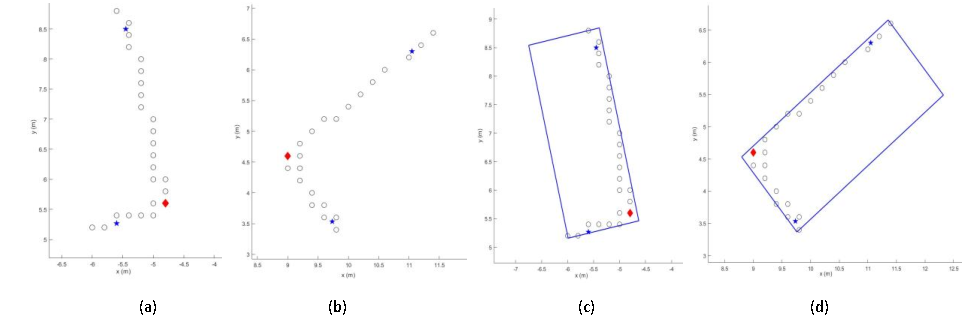
\includegraphics[width=1.0\linewidth]{figures/l_shape_fitting_fig}
    \caption{Figure 6 from~\cite{zhang2017efficient}. The key points and optimal L-Shape fitting results for two typical segmentations points clusters from a laser scanner. The blue stars and red diamonds represent key vertices which are identified by the LSF algorithm. Fig. (c) and Fig. (d) are the best L-Shape fitting results from the given point clusters (a) and (b), respectively, identifying both BEV size and orientation.}
    \label{fig:related-lsf}
\end{figure}

By regressing a rectangular shape to the bottom contour, the LSF algorithm is able to estimate orientation, BEV position and BEV size simultaneously.
In this work, we further adapt and develop this approach to stabilize size and heading estimates in complex traffic observation scenarios using tracking and the HD map.

\section{TrafficNet}
\label{sec:related-trafficnet}

The \textit{TrafficNet} detector~\cite{rezaei2021traffic} is a very thorough two-stage monocular traffic monitoring solution, encompassing both vehicle and VRU detection, tracking, speed estimation, and even road geometry prediction from satellite images.
This is illustrated in figure~\ref{fig:related-tranet}.

\begin{figure}[htb]
    \centering
    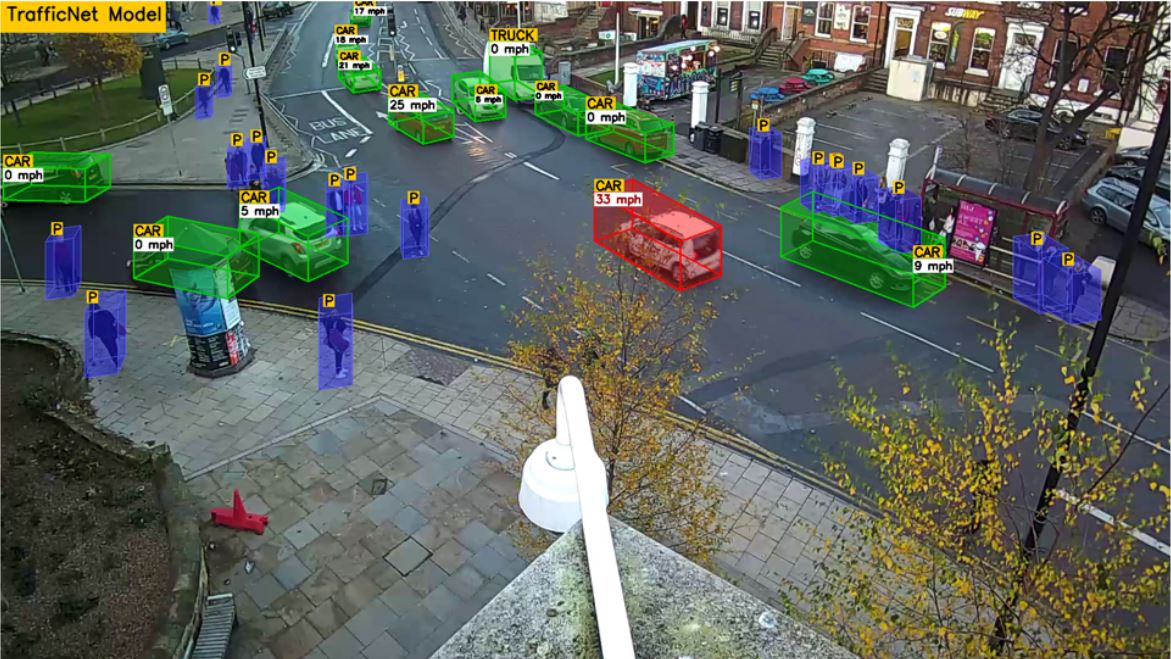
\includegraphics[width=0.63\linewidth]{figures/tranet}
    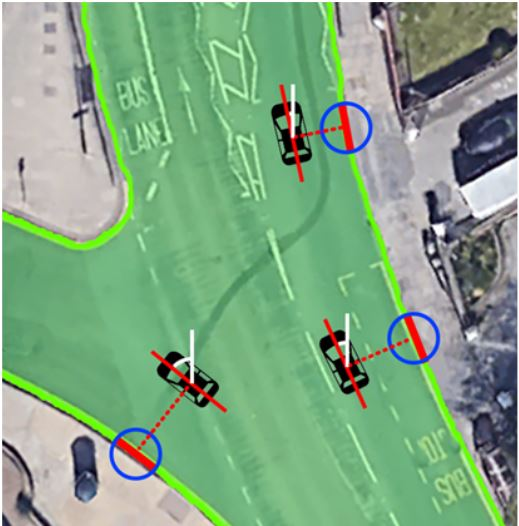
\includegraphics[width=0.35\linewidth]{figures/tranet-angle-estimation}
    %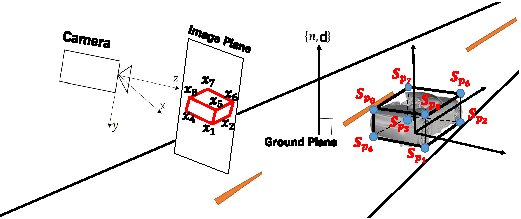
\includegraphics[width=0.39\linewidth]{figures/cvis_figure_2}
    \caption{Figures 12 and 13(c) from~\cite{rezaei2021traffic}, illustrating their approach to heading estimation based on the geometry of proximate road curbs which have been extracted from sattelite imagery. This is analogous to our use of the HD map in this work (to some extent).}
    \label{fig:related-tranet}
\end{figure}

As can be seen from the right side of figure~\ref{fig:related-tranet}, they make use of road curb geometry which is extracted from HD maps to make estimates of vehicle headings, substituting the role of the HD map in this work.
Note, that heading estimation via the most proximate curb would not be applicable in this work, as curbs within a complex intersection with many overlapping lanes are not a good indicator of orientation.
However, their approach alleviates the need for rather hard-to-source high-definition maps, which is a point of weakness in this work.
Another strong point of \textit{TrafficNet} is their extensive use of Kalman Filters~\cite{welch1995kalman} to de-noise the vehicle pose and category estimations.
They also fine-tuned a custom instance mask segmentation model in the first detector stage based on YOLOv5~\cite{glenn_jocher_2020_4154370}.
This is done both to detect additional object categories, and to speed up inference by removing convolutions which are only needed to detect large objects.
One weak point of their work is the extensive use of \enquote{magic values} in the second detector stage: They make use of pre-defined sizes based on vehicle categories, and calculate 3D object height based on a pre-calculated factor of \textit{$0.6$} from the instance mask height.
Also, unfortunately, no code is publicly available for \textit{TrafficNet}.

\section{UrbanNet: Urban Maps for Long Range 3D Object Detection}
\label{sec:related-urbnet}

Another case of a two-stage object detector which using Urban maps to augment the performance of the $2D \rightarrow 3D$ lifting-stage is \textit{UrbanNet}~\cite{carrillo2021urbannet}.
This solution is unique, because it applies the HD map as an auxiliary feature to a small Feed-Forward Neural Network.
The architecture is illustrated in figure~\ref{fig:related-urbnet}.

\begin{figure}[htb]
    \centering
    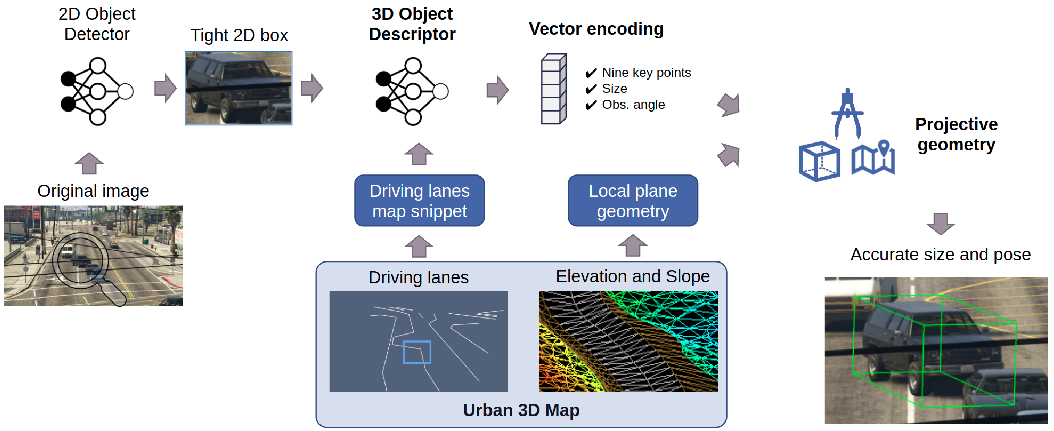
\includegraphics[width=1.0\linewidth]{figures/urbannet_architecture}
    \caption{Figure 2 from~\cite{carrillo2021urbannet}, describing how the Urban HD map assists the 3D object descriptor estimation model. Center-lines are \textit{painted} as a per-pixel feature into the 3D object descriptor network's single input image.}
    \label{fig:related-urbnet}
\end{figure}

This approach provides an interesting way to remediate some of the shortcomings of L-Shape-Fitting in the second detector stage.
The neural network can learn to recognize obstructed road user poses, or even highly uncommon poses, such as a car laying on its side in a crash scenario
This is not possible with a bottom-contour based detector.
Furthermore, the performance might actually increase, as there is no requirement for the first detector stage to compute expensive instance masks.
Notably, they also incorporate slope estimation into their prediction, which is especially useful for long-range vision in mountainous terrain.
The bottleneck in this case is the availability of training data, something which is solved in UrbanNet by training and testing exclusively on artificial computer-generated road scenes.

\section{Cooperative Roadside Vision Systems in Complex Scenarios}
\label{sec:related-crvis}

Finally, the \textit{Complex Scenario Cooperative Roadside Vision System}~\cite{masi2021augmented} is related as prior work due to its two-stage monocular 3D object detection architecture and usage of HD maps in all stages of the detection processes.

\begin{figure}[htb]
    \centering
    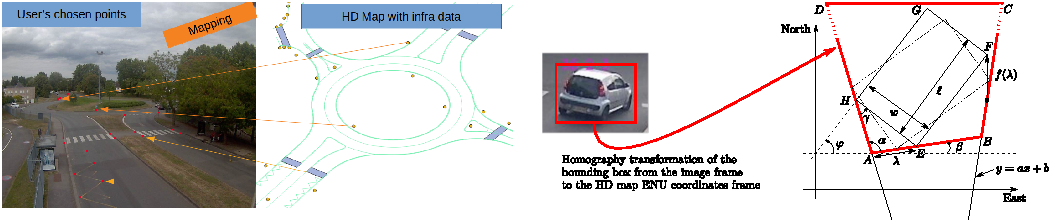
\includegraphics[width=1.0\linewidth]{figures/coop_roadside_vis_aug_perception_fig}
    \caption{Figures 2 and 3 from~\cite{masi2021augmented}, describing how the HD map is used for calibration (left) and how the vehicle size is calculated from its 2D bounding box (right).}
    \label{fig:related-crvis}
\end{figure}

Their system uses the HD map for calibration (as illustrated in figure~\ref{fig:related-crvis}), heading calculation, and tracking.
On the other hand, their paper is not clear on when and how exactly they make use of the HD-map for heading estimation.
In some or most cases, they fall back to a projection of the 2D screen-space bounding box onto the 3D ground plane, from which a vehicle's BEV width/length and heading may be calculated.
They do not make any attempts at calculating vehicle heights or detecting VRUs.

\section{Survey Studies}
\label{sec:related-surveys}

In the conclusion of this related work study, several survey papers were consulted, some of which shall be highlighted here for reference.

First of all, the survey \textit{3D Object Detection from Images for Autonomous Driving}~\cite{survey2022} was a great resource to learn a taxonomy for the multitude of architectural approaches towards the \textit{Mono3d} task.

Furthermore, the survey on \textit{Object Detection in Traffic Videos} provides an in-depth overview on the spectrum techniques which are used in 2D object detection neural networks, such as YOLO~\cite{wang2022yolov7}.

Research on \textit{Infrastructure-Based Object Detection and Tracking for Cooperative Driving Automation}~\cite{bai2022infrastructure} is very connected to this work, and the cited survey includes many of the previously mentioned related works.

Finally, the \textit{Review on Cooperative Perception and Control Supported Infrastructure-Vehicle Systems}~\cite{yu2022review} is the only survey which mentions HD maps as an auxiliary data source and shared spatial reference frame for cooperating autonomous vehicles.
